%Problem Set 1 LaTeX report for TDT4200
\documentclass[fontsize=11pt, paper=a4, titlepage]{article}
\usepackage{float} %For forcing position of figures
\usepackage{listings}	%For code in document
\usepackage[usenames,dvipsnames]{color}		%For the SkyBlue background color for lstlistings
\usepackage{mathtools}
\DeclarePairedDelimiter{\ceil}{\lceil}{\rceil}
\usepackage{amsfonts,amsmath,amssymb,amsthm}	%For \mathbb
% \usepackage{caption}	%Dunno yet
\usepackage{todonotes}	%For \todo
\usepackage{tabularx}	%for tablecontents wrapping inside cell, instead of cell breaking page width.
\usepackage{verbatim}
\usepackage{enumerate}	%For getting different types of lists like a) II) and so forth.
\usepackage[margin=2cm]{geometry}
\usepackage[utf8, utf8x]{inputenc}	%For norwegian letters and UTF8 encoding support
\usepackage{lastpage}	%For the command \pageref{lastpage}
\usepackage{fancyhdr}
\rfoot{\thepage\ / \pageref{LastPage}}

\usepackage{tikz}
\usepackage{colortbl}
\usetikzlibrary{calc}
\newcolumntype{W}{!{\smash{\vrule
\@width 4\arrayrulewidth
\@height\dimexpr\ht\@arstrutbox+2pt\relax
\@depth\dimexpr\dp\@arstrutbox+2pt\relax}}}
\makeatother
\definecolor{gray}{rgb}{.7,.7,.7}

\newcommand*\Laplace{\mathop{}\!\mathbin\bigtriangleup}

%\setlength{\parindent}{10ex}

\lstset{ %
language=C,							% choose the language of the code
basicstyle=\ttfamily,			% the size of the fonts that are used for the code
numbers=left,						% where to put the line-numbers
numberstyle=\footnotesize,			% the size of the fonts that are used for the line-numbers
stepnumber=1,						% the step between two line-numbers. If it is 1 each line will be numbered
numbersep=5pt,						% how far the line-numbers are from the code
backgroundcolor=\color{SkyBlue},	% choose the background color. You must add \usepackage{color}
showspaces=false,					% show spaces adding particular underscores
showstringspaces=false,				% underline spaces within strings
showtabs=false,						% show tabs within strings adding particular underscores
frame=single,						% adds a frame around the code
tabsize=4,							% sets default tabsize to 4 spaces
captionpos=b,						% sets the caption-position to bottom
breaklines=true,					% sets automatic line breaking
breakatwhitespace=false,			% sets if automatic breaks should only happen at whitespace
escapeinside={\%*}{*)}				% if you want to add a comment within your code
}

\lstset{literate=
	{á}{{\'a}}1 {é}{{\'e}}1 {í}{{\'i}}1 {ó}{{\'o}}1 {ú}{{\'u}}1
	{Á}{{\'A}}1 {É}{{\'E}}1 {Í}{{\'I}}1 {Ó}{{\'O}}1 {Ú}{{\'U}}1
	{à}{{\`a}}1 {è}{{\'e}}1 {ì}{{\`i}}1 {ò}{{\`o}}1 {ù}{{\`u}}1
	{À}{{\`A}}1 {È}{{\'E}}1 {Ì}{{\`I}}1 {Ò}{{\`O}}1 {Ù}{{\`U}}1
	{ä}{{\"a}}1 {ë}{{\"e}}1 {ï}{{\"i}}1 {ö}{{\"o}}1 {ü}{{\"u}}1
	{Ä}{{\"A}}1 {Ë}{{\"E}}1 {Ï}{{\"I}}1 {Ö}{{\"O}}1 {Ü}{{\"U}}1
	{â}{{\^a}}1 {ê}{{\^e}}1 {î}{{\^i}}1 {ô}{{\^o}}1 {û}{{\^u}}1
	{Â}{{\^A}}1 {Ê}{{\^E}}1 {Î}{{\^I}}1 {Ô}{{\^O}}1 {Û}{{\^U}}1
	{œ}{{\oe}}1 {Œ}{{\OE}}1 {æ}{{\ae}}1 {Æ}{{\AE}}1 {ß}{{\ss}}1
	{ç}{{\c c}}1 {Ç}{{\c C}}1 {ø}{{\o}}1 {å}{{\r a}}1 {Å}{{\r A}}1
	{€}{{\EUR}}1 {£}{{\pounds}}1
}
 %config.tex file in same directory for all reports

\begin{document}

\begin{center}

{\huge Problem Set 2}\\[0.5cm]

\textsc{\LARGE TDT4200 -}\\[0.5cm]
\textsc{\large Parallel Computations}\\[1.0cm]

\begin{table}[h]
    \centering
    \begin{tabular}{c}
        \textsc{Christian Chavez}
    \end{tabular}
\end{table}

\end{center}
\vfill
\large{\today}
\clearpage

\section{Theory}
\subsection{Problem 1, MPI}

\begin{enumerate}
\renewcommand{\theenumi}{\alph{enumi})}

    \item Blocking sends in MPI (like MPI\_Send() and MPI\_Recv()), block the
flow of the program until the corresponding rank reached the corresponding
sent/received call in its own program flow.

Non-blocking sends do not wait for the receiving rank to be ready with the
receiving buffer. Nor do the receiving ranks wait to make sure that the data has
been sent from the rank sending it. Hence, the function MPI\_Wait() can be used
to ensure that the rank does not continue its program flow with data not yet
received/ready. Or Make sure of this in some other manner.

    \item What is the difference between synchronous and asynchronous sends in MPI?
Synchronous sends require both parties to be ready and ``waiting'' for the send to be transmitted. Hence, a synchronous send can also be described as a blocking send.

Asynchronous sends can generally be described as a non-blocking send, but
depending on use of functionality like MPI\_wait() (or something likewise), it
doesn't have to be non-blocking.

\end{enumerate}

In effect, non-blocking vs blocking, and asynchronous vs synchronous are in
effect the same thing, though the implementation. The difference comes down to
semantics more often than not.

\subsection{Problem 2, Interconnects}

\begin{enumerate}
\renewcommand{\theenumi}{\alph{enumi})}

    \item
    \begin{itemize}
        \item A picture of a mesh with 16 nodes:
        \begin{figure}[H]
            \centering
            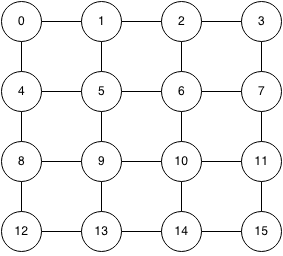
\includegraphics[width=0.4\linewidth]{16_node_mesh.png}
            \caption{16 node mesh}
            \label{fig:mesh}
        \end{figure}

        \item A picture of a torus with 16 nodes, albeit I was unable to find
out if a torus of interconnected computing nodes needs to be connected along
both dimensions, or just along the one like in the below picture.
        \begin{figure}[H]
            \centering
            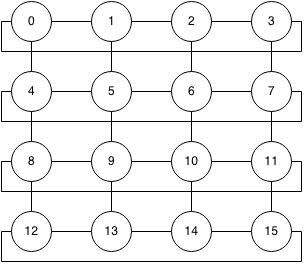
\includegraphics[width=0.4\linewidth]{16_node_torus_1d.png}
            \caption{16 node torus}
            \label{fig:torus}
        \end{figure}

        \item A picture of a hypercube with 16 nodes:
        \begin{figure}[H]
            \centering
            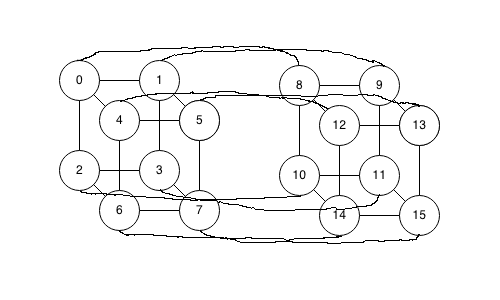
\includegraphics[width=0.8\linewidth]{16_node_hypercube.png}
            \caption{16 node hypercube}
            \label{fig:hypercube}
        \end{figure}
    \end{itemize}


    \item The biggest bisection width is the hypercube, which has a bisection
width of 8, or the torus which also has a bisection width of 8. The smalles
bisection width is the mesh, which has the bisection width of 4.

\end{enumerate}

\subsection{Problem 3, Amdahl and Gustafson}
\begin{align*}
    P_s &= \frac{P_{Size\thickspace of\thickspace the\thickspace trictly\thickspace serial\thickspace code\thickspace part\thickspace of\thickspace the\thickspace program}}{Total\thickspace size\thickspace of\thickspace the\thickspace program} \\
    P_p &= \frac{P_{Size\thickspace of\thickspace the\thickspace infinitely\thickspace parallell\thickspace code\thickspace part\thickspace of\thickspace the\thickspace program}}{Total\thickspace size\thickspace of\thickspace the\thickspace program} \\
    N &= Number\thickspace of\thickspace processes\thickspace program\thickspace is\thickspace run\thickspace on\thickspace in\thickspace parallell \\
    S_{Amdahl} &= \frac{1}{s_a + \frac{1-s_a}{n}} \\
    S_{Gustafson} &= N - \frac{P_s}{P_s + \frac{P_p}{N}}\cdot(N-1) = N - s_g\cdot (N-1)
\end{align*}

In this problem, the following values are given:
\begin{align*}
    P_s &= 0.4\thickspace seconds \\
    P_p &= 0.6\thickspace seconds \\
    N &= 10\thickspace processors
\end{align*}

\begin{enumerate}
\renewcommand{\theenumi}{\alph{enumi})}
    \item The speedup using Amdahl's law is:
    \begin{align*}
        S_a &= \frac{1}{0.4 + \frac{1-0.4}{10}} = \frac{1}{0.4+0.06} \\
        S_a &= \frac{50}{23}\thickspace seconds
    \end{align*}

    \item The speedup using Gustafson's law is:
    \begin{align*}
        S_g &= 10 - \frac{0.4}{0.4 + \frac{0.6}{10}}\cdot (10-1) = 10 - \frac{0.4}{0.46}\cdot 9 \\
        S_a &= 10 - \frac{180}{23} = \frac{50}{23}\thickspace seconds
    \end{align*}

    \item $s_a$ is the fraction of execution time that has to be done in serial,
while $s_g$ is the serial work done on $N$ processes. In essence, these two are
the same. We get the same result since Amdahl focuses on the time it takes to
execute the unparallellizable code, while Gustafson focuses on how much work can
be done serially across all the $N$ processes/machines/cores.

\end{enumerate}

\subsection{Problem 4, Communication}
\renewcommand{\theenumi}{\alph{enumi})}
\begin{align*}
    Datasize &= n\times n\thickspace 2D\thickspace array \\
    P &= m^2,\thickspace where\thickspace n > m
\end{align*}

Assumption 1: The root processor is the one that reads and distributes the
image, instead of all processors having the image at start and only working on
their subdomain of the image.

Assumption 2: When dealing with exchanges, I assume that in cases where $m^2 \%
2 != 0$, do not need to be taken into account below in c) and d). However, if
they were to be taken into account, it would imply a $+1$ on the amount of
processes. AKA $m^2$ then becomes $m^2 +1$

\begin{enumerate}

    \item Total elements sent and received from root node to distribute and gather image
    \begin{align*}
        &= (m^2 - 1)\times (\frac{n}{m})^2\times 2
    \end{align*}

    \item Amount of grid elements sent between all processes per exchange of borders
    \begin{align*}
        &= \frac{4n}{m}\times m^2\times 2 = 8n\times m
    \end{align*}

    \item Time spent on an exchange when all processes can communicate full-duplex
with no overhead at $r$ bytes/second with only one other process at a time, without any startup time per transmission
    \begin{align*}
        &= \frac{4n}{m}\times \frac{b}{2r} = \frac{2nb}{mr}
    \end{align*}


    \item Total time for execution $T$
    \begin{align*}
        T &= T_{comp} + T_{comm} \\
        T_{comp} &= t \frac{n^2}{m^2},\thickspace t\thickspace is\thickspace constant \\
        T_{comm} &= \frac{(m^2 -1)\times \frac{n^2}{m^2}\times 2}{1}\times \frac{b}{r} +  \frac{2nb}{mr} = \frac{2b}{r}\times (n^2 - \frac{n^2}{m^2} + \frac{n}{m})
    \end{align*}
    Since $\frac{2b}{r}$ is constant, this factor is henceforth referred to as $C$, hence
    \begin{align*}
        T &= C \times (n^2 - \frac{n^2}{m^2} + \frac{n}{m})
    \end{align*}

\end{enumerate}

\vfill
\large{\today}
\end{document}
